
\section{Solid scintillation detectors versus LXe}
\label{sec.ssd}

\subsection{Solid scintillation detectors}

Today's conventional PETs use solid scintillation detectors (SSD) such as Sodium Iodine (NaI), Bismuth Germanate (BGO) or Lutetium oxyorthosilicate (LSO), and Lutetium-yttrium oxyorthosilicate (LYSO) readout by light sensitive detectors. The standard has shifted from the use of NaI crystals to the use of BGO and LSO devices. Until recently, the SSDs were readout with photomultipliers (PMTs), but the so-called Silicon Photomultipliers (SiPMs) are emerging in the last few years as a major alternative. Unlike PMTs, SiPMs can be used in the presence of a strong magnetic field, therefore opening the possibility to build Nuclear Magnetic Resonance (IMR) compatible PET devices. 

The physical properties that define SSDs are: 
\begin{enumerate}
\item {\bf Attenuation length ($\lambda$)}, which sets the scale of the length (across the photon line of flight) that the detector has to have in order to stop most of the incoming radiation.
\item {\bf Density ($\rho$)}, which is related with the total size and weight of the detector.
\item {\bf Photon yield per keV ($Y$)}, which must be as high as possible to record large signals. 
\item {\bf Energy resolution at 511 keV ($\sigma_E$)}, which must be as good as possible. 
\item {\bf Transverse spatial resolution ($\sigma_T$)} (relative to the photon line of flight), which in turn depends on the photon yield and the granularity of the readout sensors.
\item {\bf Longitudinal spatial resolution ($\sigma_L$)}, important to minimize the so-called parallax error.  $\sigma_L$~  tends to be poor for the SSDs, which do not measure the longitudinal coordinate (thus $\sigma_L \sim L/\sqrt{12}$, where $L$~is the detector length). 
\item {\bf Scintillation decay time ($t_s$)}, which must be as fast as possible, to maximize the number of events acquired per unit time and to minimize the window used to correlate events in different crystals. In addition, if the system has very good time resolution (in the range of few hundred picoseconds) time-of-flight measurements (TOF) are possible.  
\end{enumerate}

\subsection{Liquid Xenon as detection material}

%
%\begin{figure}[!bhtp]
%	\centering
%	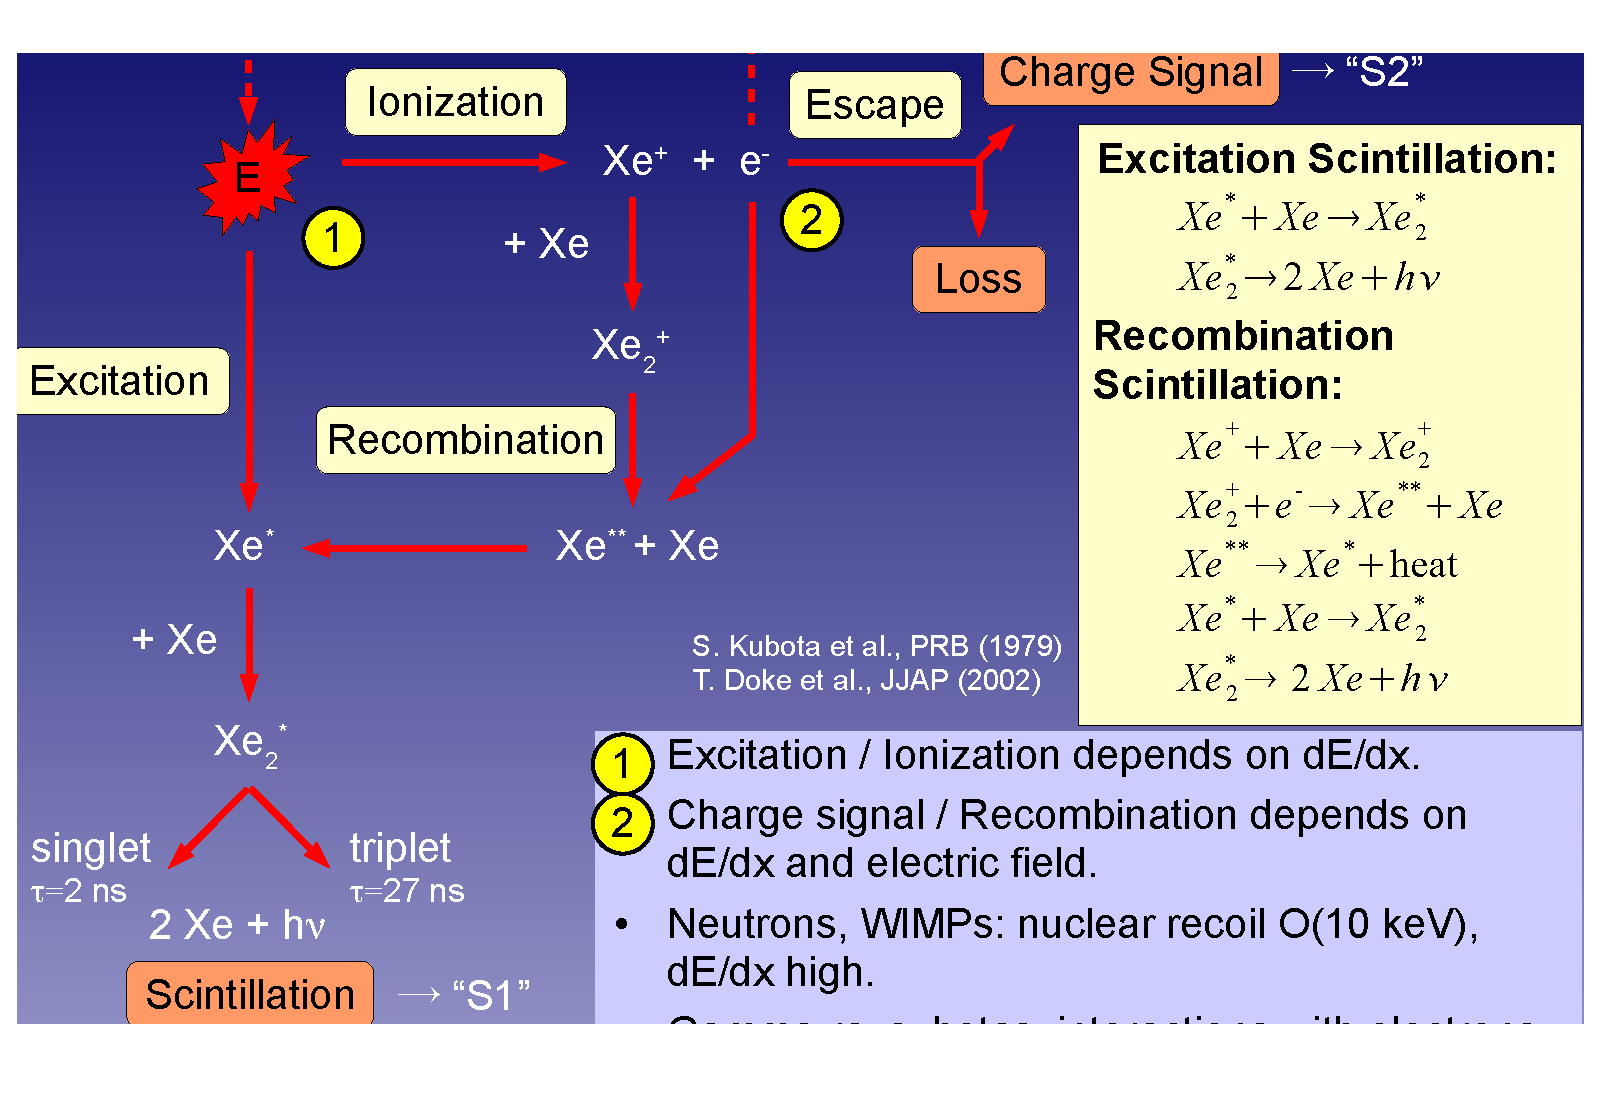
\includegraphics[scale=0.5]{img/XeLight.pdf}
%	\caption{\label{fig.xel} Scintillation and ionization properties of LXe.}
%\end{figure}

Xenon is a noble gas. It responds to ionizing radiation providing both ionization and scintillation signals. The ionization signal is due to atomic electrons ejected from the xenon atoms by the incoming radiation, which take a long time to recombine due to the noble-gas nature of xenon (and therefore can be drifted to a collection electrode, if so desired). The scintillation signal is due to the de-excitation of xenon atoms forming dimers which decay after 2.2 ns (dominant single mode) or 27 ns (triplet mode) emitting ultraviolet light (VUV) of 178 nm wavelength %(Figure \ref{fig.xel}).

If $E$~ is the energy deposited by the ionizing radiation (in this case 511 keV), the maximum scintillation yield of LXe is given as $E/W_{ph}$, where $W_{ph}$~ is the average energy required for the production of a single photon. The most probable value of $W_{ph}$~ in LXe  is  $13.8 \pm 0.9$~eV \cite{aprile10}. Therefore, a maximum of 37,000 scintillation photons are produced when a 511 keV gamma interacts in the LXe. On the other hand, measurements carried out with electrons of 1 MeV result in a value of $W_{ph}^e = 21.6$ \cite{doke02}. This value is attributed to ionization electrons that do not recombine, and would imply a yield of $\sim$ 24,000 scintillation photons for a 511 keV gammas. The results presented in this work are obtained assuming the maximum scintillation yield, but we also discuss the implications of a lower scintillation yield in the energy and spacial resolution. 

In its liquid phase (at a temperature of 165 K and 1 bar of pressure) LXe has a reasonable high density (3 g/cc) and an acceptable attenuation length for 511 keV gammas (36 mm), which makes it suitable for PET applications. Its advantage with respect to SSD are: a) its very high yield (24,000--37,000 photons for a 511 keV gamma), which in turn can translate in excellent energy and transverse spatial resolution; b) Its ability to provide a 3D measurement of the interaction point and thus a high-resolution measurement of the longitudinal coordinate, minimizing parallax errors; c) its capability to identify Compton events depositing all its energy in the detector as separate-site interaction, due to the relatively large interaction length in xenon;  d) its very fast scintillation decay time, which makes it suitable as a TOF-PET;  and e) its relatively low cost (e.g, about 10\% of the cost of LSO per unit detector).  Table \ref{table.SDPP} shows the physical properties of common PET SSD compared with that of liquid xenon (LXe). 


\begin{table}[htdp!]
\caption{Physical properties of common PET SSD and of LXe}
\begin{center}
\begin{tabular}{l|cccc}
\toprule
& \textbf{NaI} & \textbf{BGO} & \textbf{LSO} & \textbf{LXe}\\
\hline
Effective $Z$ & 50 & 74 & 66 & 54 \\
$\rho$~(g/cm$^3$) & 3.7 & 7.1 & 7.4 &  3 \\
$\lambda$ ~ at 511 keV (mm) & 28 & 11 & 12 & 36 \\
$Y$~per keV & 38 & 6 & 29 & {\bf 72.4} \\
%RLO & 100 & 15 & 75 & {\bf 190} \\
$t_s$~(ns) & 230 & 300 & 40 & {\bf 2.2} \\
\toprule
\end{tabular}
\end{center}
\label{table.SDPP}
\end{table}%
